Solve the heat equation $u_{xx} = u_t$ on the domain $\Omega = [0, \pi]$ with initial temperature distribution 
$u(x, 0) = x$ and Dirichlet boundary conditions $u(0, t) = u(\pi, t) = 0$.

\begin{solution}\ \\\\
    Let $L = \pi$. We begin with the observation that the fact that our boundary conditions are fixed to zero implies 
    that our steady-state solution $u_s(x)$ is identically zero. Hence we need only solve for the transient solution 
    $v(x, t)$.  To do so, we utilize separation of variables and assume that $v(x, t)$ is the product of some function 
    of $x$ and some function of $t$, i.e., $v(x, t) = \phi(x) G(t)$. Substituting the product form of $v(x, t)$ into the
    heat equation yields:

    $$
    \frac{\partial^2}{\partial x^2} (\phi(x) G(t)) = \frac{\partial}{\partial t} (\phi(x) G(t)) \\
    $$

    and hence (observing that the partial derivatives on either side reduce to standard derivatives):

    $$
    G \frac{d^2 \phi}{d x^2} = \phi \frac{d G}{d t}.
    $$

    We divide both sides by $\phi G$ to find:

    $$
    \frac{1}{\phi} \frac{d^2 \phi}{d x^2} = \frac{1}{G} \frac{d G}{d t}.
    $$

    Since the left-hand side depends on $x$ only and the right-hand side on $t$, the left and right sides must be equal
    to some constant, which we denote $-\lambda^2$.

    The time-dependent side therefore becomes the first-order ODE:

    $$
    \frac{d G}{d t} = -\lambda^2 G.
    $$

    with solutions for any particular $\lambda$ given by:\footnote{
        We add subscripts here to $d_{\lambda}$ and $G_{\lambda}$ in order to emphasize that the exact form of the 
        function depends on the particular value which $\lambda$ takes.
    }

    \begin{equation}
    G_{\lambda}(t) = d_{\lambda}e^{-\lambda^2 t}.
    \end{equation}

    Similarly, the space-dependent side becomes the following second-order ODE:

    $$
    \frac{d^2 \phi}{d x^2} = -\lambda^2 \phi.
    $$

    with the following general solution (where coefficient values again depend on $\lambda$):

    $$
    \phi(x) = b_{\lambda} sin(\lambda x) + c_{\lambda} cos(\lambda x).
    $$

    Our boundary condition $0 = u(0, t) = \phi(0)$ yields:

    $$
    0 = \phi(0) = b_{\lambda} sin(0) + c_{\lambda} cos(0) = c_{\lambda}.
    $$

    Similarly, our boundary condition $0 = u(L, t) = \phi(L)$ yields:

    $$
    0 = \phi(L) = b_{\lambda} sin(\lambda L).
    $$

    Since we assume a non-trivial solution, we have that $\lambda$ must be:

    $$
    \lambda_n = \frac{n \pi}{L}, n \in \mathbb{N}
    $$

    Hence for any particular $n$, we have that $u_n(x, t) = \phi_n(x)G_n(t)$ is a solution to our PDE. Because arbitrary
    linear combinations of solutions are themselves solutions to the PDE by the principle of superposition, we have that
    our solution $u(x, t)$ is given by:

    \begin{equation}
    u(x, t) = \sum\limits_{n=1}^{\infty}{b_n \sin\left(\frac{n \pi x}{L}\right)} d_n e^{-\left(\frac{n \pi}{L}\right)^2 t}
            = \sum\limits_{n=1}^{\infty}{a_n \sin\left(\frac{n \pi x}{L}\right)} e^{-\left(\frac{n \pi}{L}\right)^2 t}.
    \end{equation}

    To determine our Fourier sine coefficients $a_n$, we substitute (2) into our initial condition $u_0(x) = x$:

    \begin{align*}
        x = u_0(x) = u(x, 0) = \sum\limits_{n=1}^{\infty}{a_n \sin\left(\frac{n \pi x}{L}\right)}.
    \end{align*}

    We multiply each side by $\sin\left(\frac{m \pi x}{L}\right)$ for some fixed $m \in \mathbb{N}$ and integrate over 
    our domain $\Omega$ to find:\footnote{
        We may switch the order of integration and summation by the Dominated Convergence Theorem.
    }

    \begin{align*}
        \int_{0}^{L}{u_0(x) \sin{\left(\frac{m \pi x}{L}\right)}} 
            &= \int_{0}^{L}{\sum\limits_{n=1}^{\infty}{a_n \sin\left(\frac{n \pi x}{L}\right) \sin\left(\frac{m \pi x}{L}\right) }} \\
            &= \sum\limits_{n=1}^{\infty}{a_n \int_{0}^{L}{\sin\left(\frac{n \pi x}{L}\right) \sin\left(\frac{m \pi x}{L}\right) }} \\
            &= \frac{L}{2} a_m.
    \end{align*}

    Our Fourier sine coefficients are therefore given by:

    \begin{align*}
        a_m &= \frac{2}{L} \int_{0}^{L}{u_0(x) \sin{\lambda_m x}} \\
            &= \frac{2}{L} \int_{0}^{L}{x \sin{\lambda_m x}} \\
            &= \frac{2}{L} \left( -\frac{x \cos{\lambda_m x}}{\lambda_m} \bigg\rvert_{0}^{L} + \frac{1}{\lambda_m} \int_{0}^{L}{\cos{\lambda_m x}} \right) \\
            &= \frac{2}{L} \left( -\frac{x \cos{\lambda_m x}}{\lambda_m} + \frac{\sin{\lambda_m x}}{\lambda_m^2} \bigg\rvert_{0}^{L} \right) \\
            &= \frac{2}{L} \left( -\frac{L \cos{m \pi}}{\lambda_m} + \frac{\sin{m \pi}}{\lambda_m^2} \right) \\
            &= \frac{2}{L} \left( -\frac{L (-1)^m}{\lambda_m} \right) \\
            &= \frac{2 L}{m \pi} (-1)^{m+1} \\
    \end{align*}

    Substituting this expression into our full solution (2) yields our full solution $u(x, t)$:
    
    $$
    u(x, t) = \sum\limits_{n=1}^{\infty}{\frac{2 L}{n \pi} (-1)^{n+1} \sin\left(\frac{n \pi x}{L}\right)} e^{-\left(\frac{n \pi}{L}\right)^2 t}.
    $$

    For completeness, we plot two Fourier Series approximations to $u_0(x) = x$ below: \\

    \begin{figure*}[h]
        \centering
        \begin{subfigure}[b]{0.475\textwidth}
            \centering
            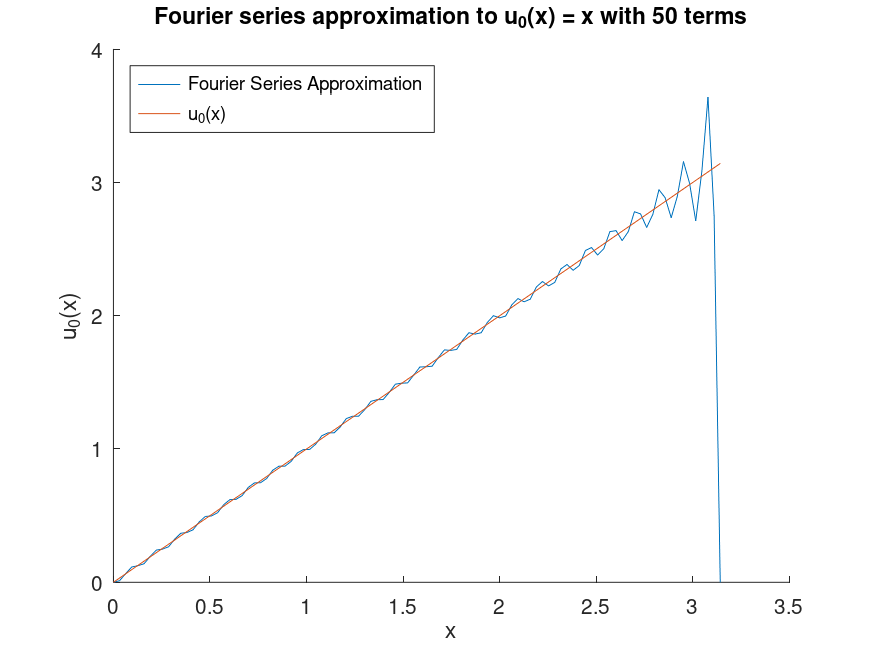
\includegraphics[width=\textwidth]{problem1_fourier_series_solution_50_terms.png}
            \label{fig:problem1_50terms}
        \end{subfigure}
        \hfill
        \begin{subfigure}[b]{0.475\textwidth}
            \centering
            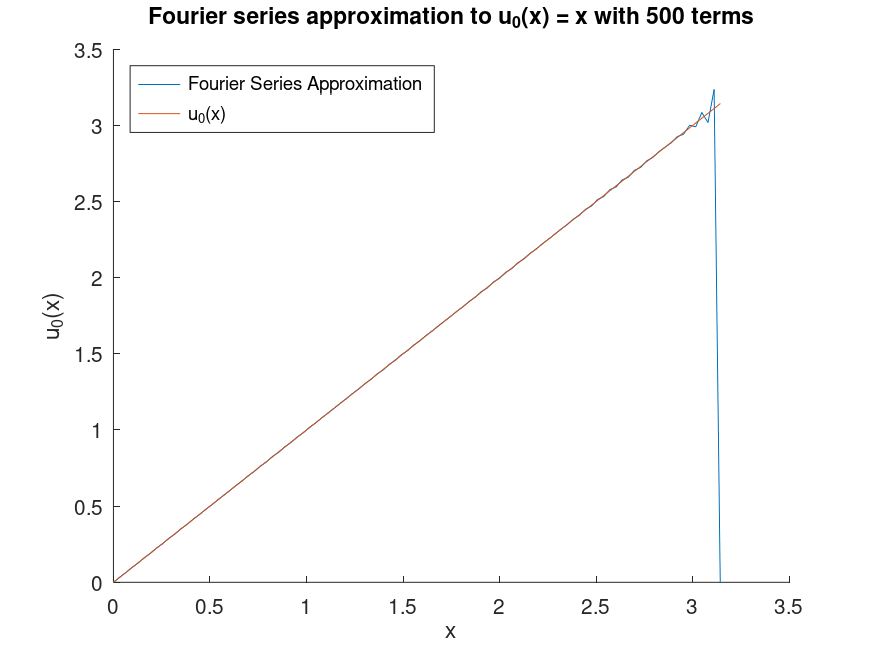
\includegraphics[width=\textwidth]{problem1_fourier_series_solution_500_terms.png}
            \label{fig:problem1_500terms}
        \end{subfigure}
        \caption[Fourier Series solution]
        {\small Fourier Series approximation to $u_0(x) = x$} 
        \label{fig:fouriersoln}
    \end{figure*}

    \pagebreak

    \lstinputlisting[style=Matlab-editor]{problem_1.m}
\end{solution}